\chapter{Metodologia}

O estudo da interface água metal foi dividido em duas etapas de simulações computacionais atomísticas: cálculos com e sem presença de um potencial externo. A primeira etapa foi realizada no código \textit{Siesta}\cite{siesta} e os cálculos envolvendo a aplicação de um potencial externo sobre a interface foram realizados no código \textit{Transiesta}\cite{transiesta1,transiesta2,transiesta3} que está baseado no \textit{Siesta}. Os elétrons do caroço foram descritos por pseudopotenciais definidos a partir do Método da Norma Conservada de \textit{Troullier-Martins} \cite{troullier_martins}. Os elétrons de valência foram expandidos em bases locais \textit{duplo-zeta polarizadas} (DZP)\footnote{Mais detalhes sobre expansões em bases atômicas localizadas e utilização de pseudopotenciais estão descritos no Apêndice \ref{apd:bases}. Os raios de corte referentes à base e ao pseudopotencial de cada elemento estão descritos no Apêndice \ref{apd:metal}.}. Em relação aos funcionais de troca e correlação, foram utilizados os funcionais PBE \cite{PBE} e VDW-BH\cite{vdw-bh}. 

Na primeira etapa, foi investigado a adsorção de duas estruturas de água, monômero e camada, sobre superfícies metálicas de Pd(111). Em particular, foi realizado primeiramente uma análise sistemática sobre parâmetros fundamentais em um cálculo atomístico, tais como a base atômica, o pseudopotencial, o funcional de troca e correlação, o tamanho da célula unitária e a quantidade de pontos k. Em seguida, foram investigadas as interações entre a água e o metal, além das interações do tipo água-água, através da minimização do sistema. Para isso, utilizou-se o algoritmo de otimização \textit{Gradiente Conjugado} com o critério de convergência para a força de $0.005\,\si{\eV}/\si{\angstrom}$ para os monômeros com orientações perpendiculares à superfície (\textit{down} e \textit{up}) e camadas de água; para o monômero orientado paralelamente ao metal (\textit{flat}) o critério foi de $0.001\,\si{\eV}/\si{\angstrom}$. O espaçamento da malha no espaço real foi de 500 Ryd. Uma vez obtida as coordenadas minimizadas, analisou-se a estabilidades das estruturas adsorvidas através das medidas geométricas, energias de adsorção e modos normais de vibração. 

Na segunda parte, utilizamos o formalismo de NEGF com DFT para aplicar uma diferença de potencial à interface água/metal, cujas superfícies metálicas foram o Pd(111) e Au(111). Por meio dessa metodologia, analisamos como as propriedades eletrônicas e vibracionais -- obtidas anteriormente para o sistema em equilíbrio -- são modificadas na presença de um potencial externo. Nessa abordagem o sistema contendo a região central e os eletrodos metálicos se encontram fora do equilíbrio termodinâmico e os eletrodos são tratados como semi-infinitos. Em relação à superfície metálica de Au, os eletrodos construídos possuíam 3 camadas com 12 átomos em cada camada ao passo que, para o sistema constituído de Pd, os eletrodos eram compostos por 6 camadas. Essa diferença no número de camadas é devido ao tamanho da base necessária para descrever o Pd. As superfícies metálicas eram separadas a fim de minimizar as interações por um vácuo de $20\,\si{\angstrom}$ no caso do eletrodo de Au e $25\,\si{\angstrom}$ para o Pd. 

Devido à sensibilidade em descrever o sistema fora do equilíbrio é necessário minimizá-lo, primeiramente, por meio de um cálculo periódico no equilíbrio até atingir o critério de força de $0.005\,\si{\eV}/\si{\angstrom}$ - como esquematizado na Figura \ref{fig:neq_flux}. Uma vez minimizado o sistema, iniciavam-se os cálculos fora do equilíbrio obtendo-se a matriz hamiltoniana e de \textit{overlap} dos eletrodos por meio de um cálculo de \textit{bulk}. Com isso, determinava-se a correção do potencial de Hartree necessário para alinhar o potencial do sistema completo com os eletrodos. Essas foram as etapas preliminares realizadas para as superfícies metálicas de Au e Pd, nos quais eram adsorvidos uma molécula ou uma camada de água. 

Em seguida, o sistema era minimizado na situação fora do equilíbrio com o potencial externo de $ 0.0\,\si{\eV} $ aplicado. Isso permitiu comparar as diferenças provocadas na interface água/metal ao descrever o metal como semi-infinito ou finito e periódico. Após essa etapa, o sistema era minimizado com o potencial externo sendo aplicado e variando entre $ V $\footnote[7]{O valor de V considerado corresponde ao potencial aplicado sobre cada eletrodo e equivale à metade do potencial total. Assim, os valores de potenciais utilizados correspondem a V/2. A mesma observação se aplica para a seção de Resultados.}=-5 a $\,5\,\si{\eV} $. Com as coordenadas minimizadas, os modos normais de vibração eram calculados pelo método de diferenças finitas \cite{phonons}. A presença de possíveis transferências de carga entre a água e o metal, bem como as interações existentes foram estudadas por meio da diferença de densidade de carga entre o potencial aplicado e o potencial igual a $ 0.0\,\si{\eV} $.

\begin{figure}[h!]
	\centering
	\caption{Fluxograma ilustrando o processo utilizado para estudar a interface água/metal no código Transiesta.}
	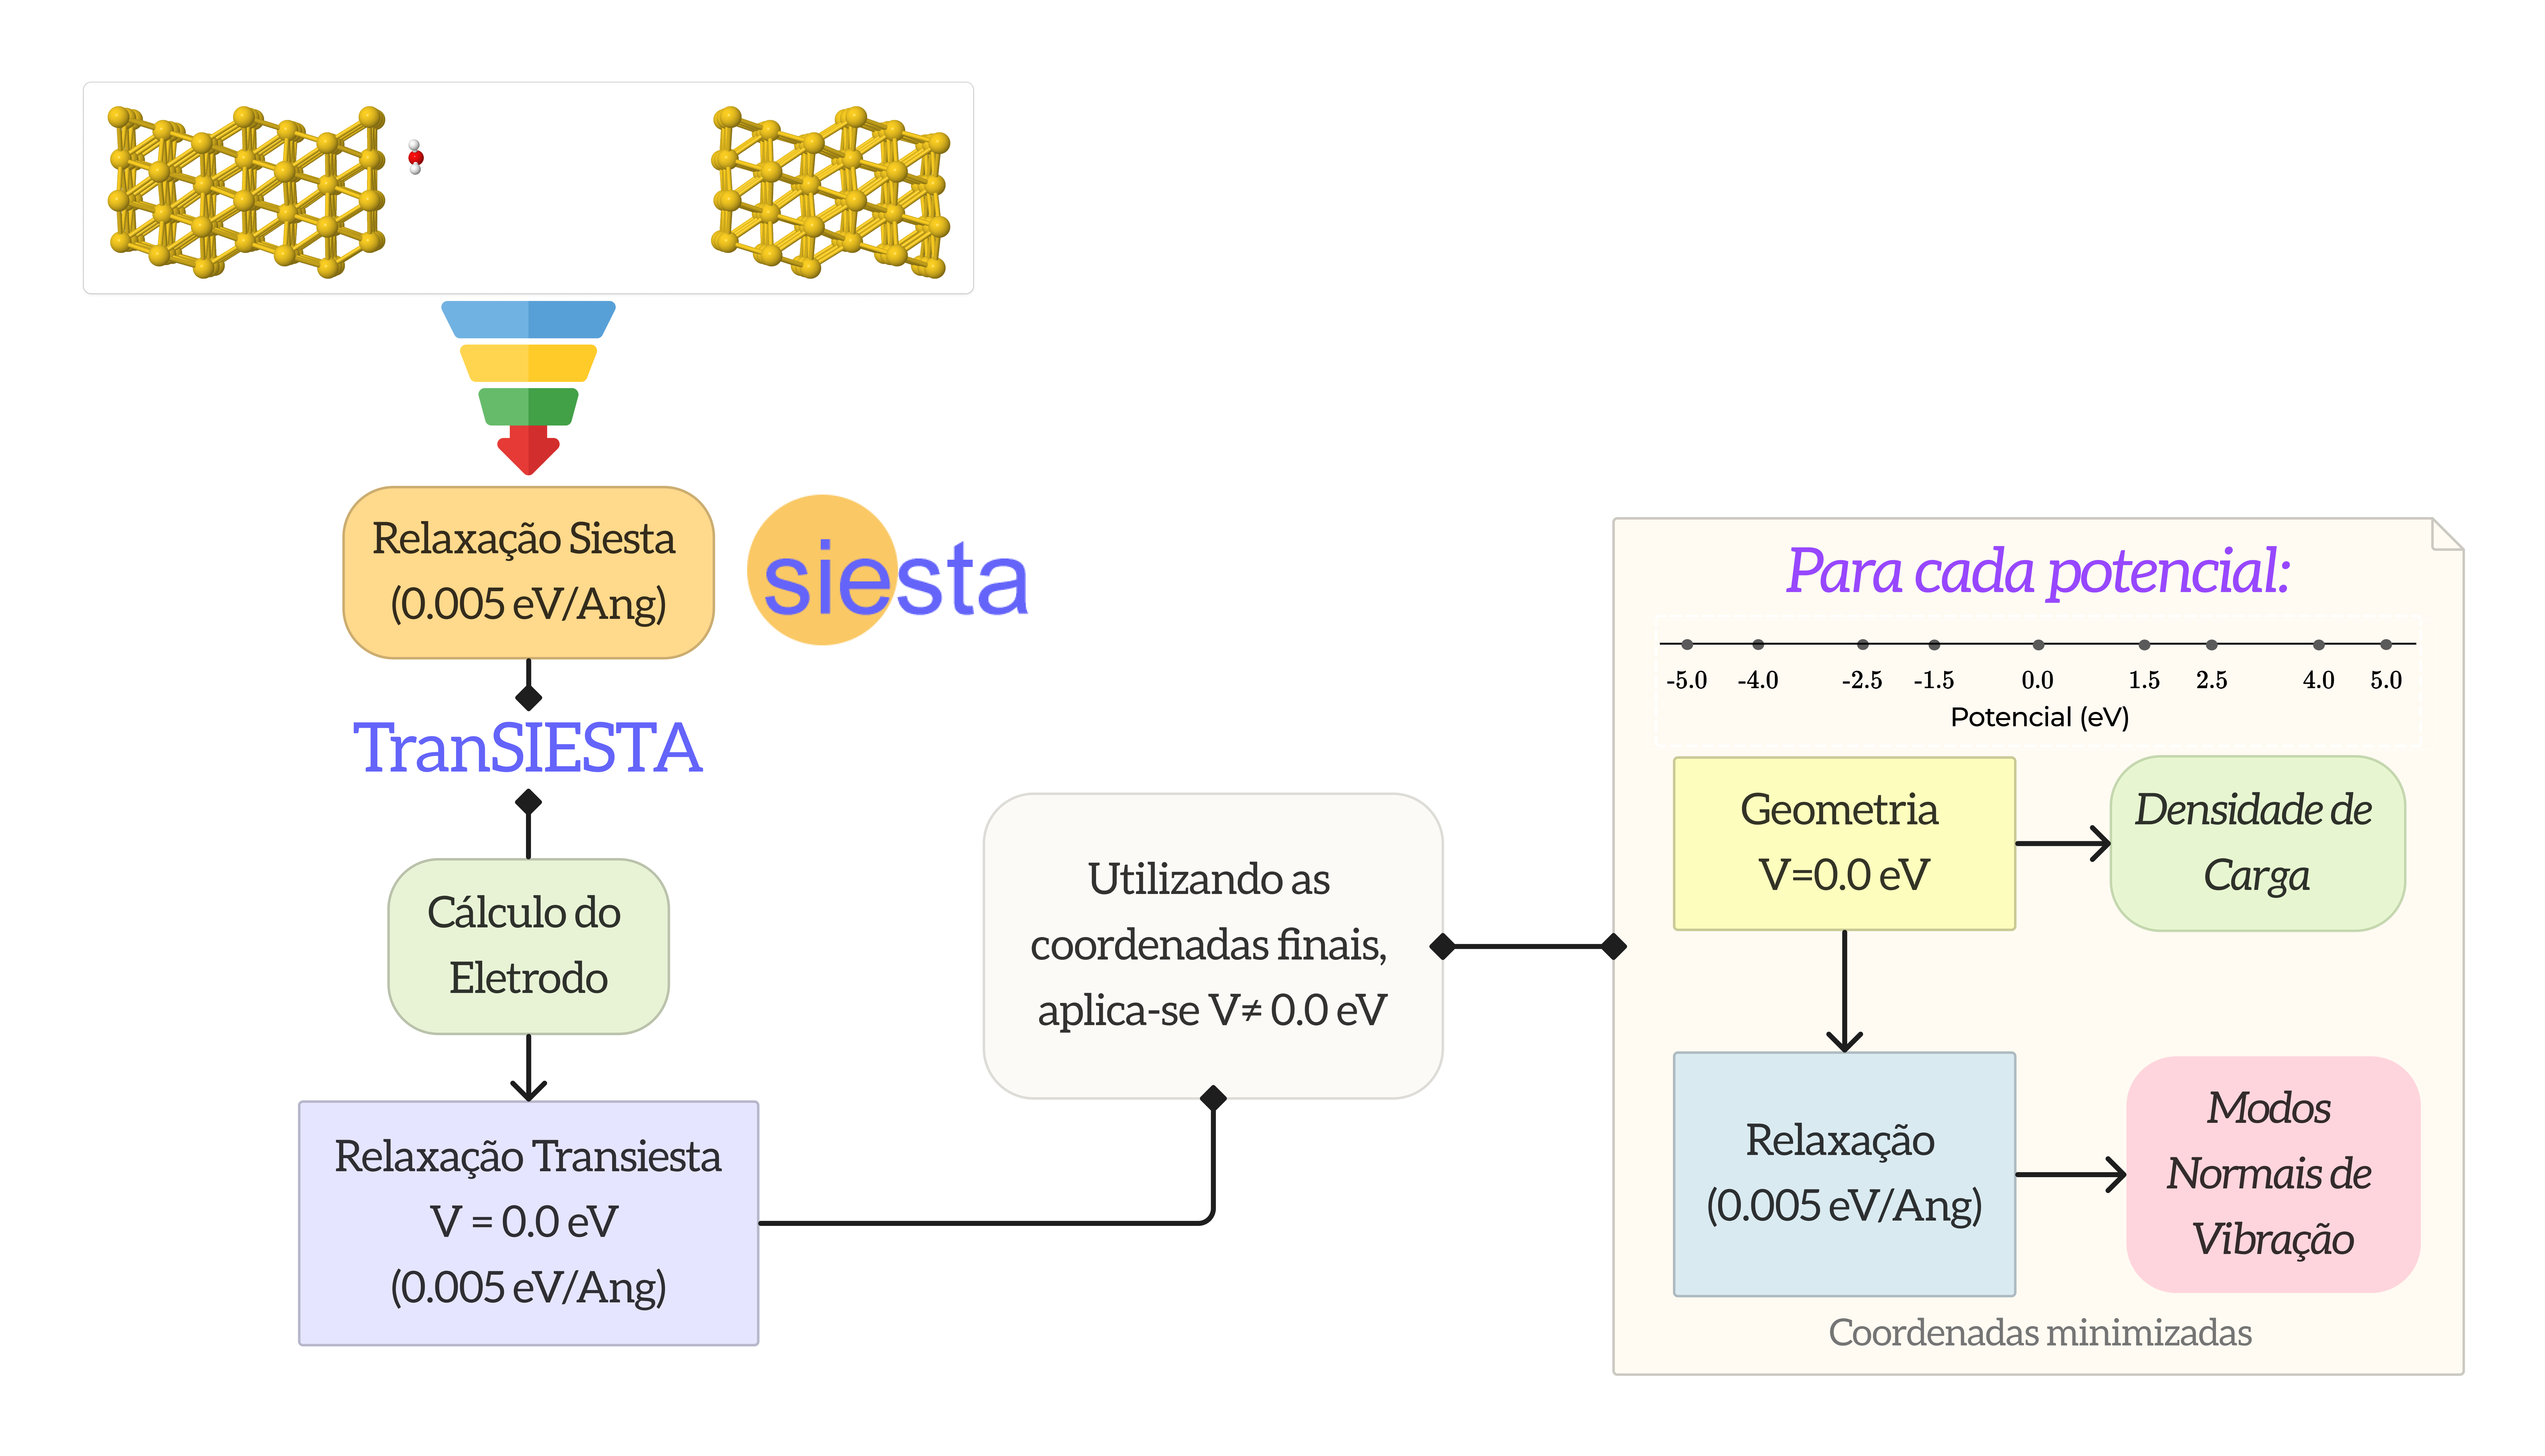
\includegraphics[scale=0.1]{figs/neq_fluxo.png}
	\legend{Fonte: compilação da autora.}
	\label{fig:neq_flux}
\end{figure} 


%Por meio das etapas descritas acima, faremos uma análise detalhada sobre o impacto da escolha de parâmetros fundamentais em um cálculo atomístico, tais como a base atômica, o pseudopotencial, o funcional de troca e correlação, o tamanho da célula unitária e a quantidade de pontos k. Além disso, obteremos parâmetros macroscópicos tais como valor da Função Trabalho e microscópicos - Modos Normais de Vibração - mediante cálculos de primeiros princípios.

